
% This file is documented here:
%   https://github.gatech.edu/math-course-repo/math-core/blob/master/docs/slides.md

% Set this before compiling anything at all.
% Format is MM-DD.
\ifdefined\lecturedate\else
\def\lecturedate{}
\fi

%----------------------------------------------------------------------
% Configure compilation parameters based on what file is being compiled
%----------------------------------------------------------------------
\def\texingmode{texing}  % Currently working on the file
\def\classmode {class}   % Presentation mode for in class
\def\webmode   {web}     % Handout mode for the website
\def\blankmode {blank}   % Handout mode for the website, with blank webonly
\def\minemode  {mine}    % Two-page mode with instructor \note{}s

%\let\slidesmode=\minemode

\ifx\slidesmode\classmode
\message{Compiling in presentation mode for in-class slides}
\def\outputmode{presentation}
\else\ifx\slidesmode\webmode
\message{Compiling in handout mode for the website}
\def\outputmode{handout}
\else\ifx\slidesmode\blankmode
\message{Compiling in handout mode for the website (blank webonly)}
\def\outputmode{handout}
\else\ifx\slidesmode\minemode
\message{Compiling in two-page mode with instructor notes}
\def\outputmode{handout}
\else
\message{Compiling in presentation mode with transparent webonly}
\def\outputmode{presentation}
\let\slidesmode=\texingmode
\fi\fi\fi\fi

\documentclass[xcolor=table,9pt,t,\outputmode,usepdftitle=false]{beamer}
\hypersetup{pdftitle={[interactive] Linear Algebra}}

\usepackage{extarrows}
\usepackage{jdr-linalg}
\usepackage{bbding, pgfcalendar}
\newcommand\bigcheck[1][\;]{\smash{\hbox{\Huge\raise-.7ex\hbox to 0pt{%
      #1\color{seq-green}\CheckmarkBold\hss}}}}
\newcommand\bigcross[1][\;]{\smash{\hbox{\Huge\raise-.7ex\hbox to 0pt{%
      #1\color{seq-red}\XSolidBrush\hss}}}}

\usetikzlibrary{positioning,fit}
\graphicspath{{figures-slides/}{.}}

%----------------------------------------------------------------------
%-- Beamer setup
%----------------------------------------------------------------------
% Looks like GATech colors
\usecolortheme{wolverine}
% Get rid of the navigation links at the bottom of every slide
\beamertemplatenavigationsymbolsempty

%----------------------------------------------------------------------
%-- Compile mode setup
%----------------------------------------------------------------------
\usepackage{pgfpages}
\ifx\slidesmode\minemode
\setbeameroption{show notes on second screen}
\fi

\makeatletter
% Hack: redefine these so \setbeamercovered{transparent} doesn't produce glue
\define@key{beamer@mixin}{invisible}[]{%
  \def\beamer@uncoverbeforeactions{\ignorespaces}%<-- added
  \def\beamer@uncoverafteractions{\ignorespaces}}
\define@key{beamer@mixin}{transparent}[15]{%
  \def\beamer@uncoverbeforeactions{\ignorespaces\opaqueness<1->{#1}}%<-- added
  \def\beamer@uncoverafteractions{\ignorespaces\opaqueness<1->{#1}}}
\makeatother

% Show the contents of \webonly{} as transparent, for instructor's benefit
\def\transparentwebonlys{
  \def\webonlyvisible{\setbeamercovered{transparent}}
  \def\webonlyspec{0| handout:0}
  }

\ifx\slidesmode\minemode
  \transparentwebonlys
\else\ifx\slidesmode\texingmode
  \transparentwebonlys
\else\ifx\slidesmode\blankmode
  \def\webonlyvisible{}
  \def\webonlyspec{0| handout:0}
\else
  % Hide the contents of \webonly{}
  \def\webonlyvisible{}
  \def\webonlyspec{0}
\fi\fi\fi

%----------------------------------------------------------------------
%-- Overlay macros
%----------------------------------------------------------------------

% Use \webonlycmd{} or \begin{webonly}...\end{webonly} for material to write on
% the blackboard during lecture.  It won't appear on class slides, but it'll be
% semi-transparent on the instructor slides, and fully revealed on the web
% slides.
\newcommand{\webonlycmd}[1]{{%
  \webonlyvisible\uncover<\webonlyspec>{#1}}}
\newenvironment{webonly}{%
  \begingroup\webonlyvisible\begin{uncoverenv}<\webonlyspec>}%
  {\end{uncoverenv}\endgroup}

% \blankuntil{6}{blah} produces an underline with the length of ``blah''
% until slide 6, when it's replaced by ``blah'' (with no underline).
\newcommand{\blankuntil}[2]{{%
  \count255=#1\advance\count255 by -1 %
  \only<-\the\count255| handout:0>{\underline{\phantom{#2}}}%
  \advance\count255 by 1 %
  \only<\the\count255->{#2}}}

%----------------------------------------------------------------------
%-- Chapter and section titles
%----------------------------------------------------------------------

% Produces a title frame with title #1 and subtitle #2
\def\titleframe#1#2{
  \begin{frame}
    \begin{center}
      \vfill
      \structure{{\Huge\strut #1}}
      
      \bigskip
      
      \structure{\LARGE\strut #2}
      \vfill
    \end{center}
  \end{frame}
  }

%----------------------------------------------------------------------
%-- For polls
%----------------------------------------------------------------------

% Just makes a frame and sets the title.
\newenvironment{pollframe}{%
  \begin{frame}%
  \frametitle{Poll}%
  }{%
  \end{frame}%
  }

% Environment for poll material that should be hidden in blank mode
\ifx\slidesmode\blankmode
\newenvironment{poll}{%
  \begin{uncoverenv}<0| handout:0>%
  }{%
  \end{uncoverenv}%
  }
\else
\newenvironment{poll}{}{}
\fi

% Enumerate with letters A B C D etc.
\newenvironment{eAlpherate}%
  {\begin{enumerate}%
    \renewcommand{\theenumi}{\Alph{enumi}}}%
  {\end{enumerate}}

%----------------------------------------------------------------------
%-- Spacing
%----------------------------------------------------------------------
\newcommand{\displayskips}[1]{%
  \abovedisplayshortskip=#1\abovedisplayskip=#1\belowdisplayskip=#1}

%----------------------------------------------------------------------
%-- Theorem environments
%----------------------------------------------------------------------
\theoremstyle{definition}
\newtheorem{thm}{Theorem}
\newtheorem{cor}{Corollary}
\newtheorem{lem}{Lemma}
\newtheorem{eg}{Example}
\newtheorem{noneg}{Non-Example}
\newtheorem{defn}{Definition}
\newtheorem{fact2}{Fact}
\newtheorem{ques}{Question}
\newtheorem{rem}{Remark}
\newtheorem{imp}{Important}

% \begin{oneoffthm}{Big Theorem} blah \end{oneoffthm} produces
%   Big Theorem. blah
\newcounter{jdrthmtype}
\newenvironment{oneoffthm}[2][definition]{%
  \addtocounter{jdrthmtype}{1}%
  \theoremstyle{#1}%
  \newtheorem{oneoff\thejdrthmtype}[subsection]{#2}%
  \begin{oneoff\thejdrthmtype}}{%
  \end{oneoff\thejdrthmtype}}

%----------------------------------------------------------------------
%-- Emphasis box
%----------------------------------------------------------------------
\tikzset{
  bluebox/.style={draw=black, fill=blue!5, very thick, rectangle,
    rounded corners, inner sep=10pt, inner ysep=10pt, font=\normalsize},
  redbox/.style={draw=red, very thick, rounded corners, inner sep=5pt,
    font=\normalsize},
  orangebox/.style={draw=orange, thick, rounded corners, inner sep=1mm,
    font=\normalsize},
  fancytitle/.style={draw=black, fill=blue!10, text=black},
}

% Mandatory argument is the width
% Optional argument is the box title, e.g. ``Poll''
\newenvironment{bluebox}[2][]%
  {\begin{center}\begin{tikzpicture}[every node/.style={}]%
     \def\boxtitle{#1}%
     \node[bluebox](box)\bgroup%
     \begin{minipage}{#2}}%
  {\end{minipage}\egroup;%
   \ifx\boxtitle\empty\else%
     \node[fancytitle, right=10pt] at (box.north west) {\boxtitle};%
   \fi\end{tikzpicture}\end{center}}


%----------------------------------------------------------------------
%-- TikZ pictures
%----------------------------------------------------------------------
\tikzset{
  pics/gear/.style args={#1/#2}{
    code = { % #1 = number of gears, #2 = tooth length
      \filldraw[fill=black!30] (1cm-#2/2,0)
        let \n{angle} = {360/#1} in
          \foreach \gear [evaluate=\gear as \startangle using \gear*\n{angle}]
              in {1,...,#1}
            {
              arc[radius=1cm-#2/2, start angle=\startangle-\n{angle},
                  delta angle=\n{angle}/4]
              -- (\startangle-3*\n{angle}/4+\n{angle}/10:1cm+#2/2)
              arc[radius=1cm+#2/2,
                  start angle=\startangle-3*\n{angle}/4+\n{angle}/10,
                  end angle  =\startangle-  \n{angle}/4-\n{angle}/10]
              -- (\startangle-  \n{angle}/4:1cm-#2/2)
              arc[radius=1cm-#2/2, start angle=\startangle-\n{angle}/4,
                  delta angle=\n{angle}/4]
            };
          \draw (0,0) circle[radius=.4cm];
        }
    },
  % machine is an input/output machine for illustrating functions
  machine/.pic = {
    \filldraw[rounded corners=.3mm, fill=steel!30] (1.5, -1) 
      -- (1.5, -.5) -- (1.5-.2, -.5) -- (1.5-.2, .4) -- (1.5, .4)
      -- (1.5, 1) -- (-1.5, 1) -- (-1.5, -1) -- cycle;
    \filldraw[fill=steel!30] (-1.5, -.2)
      -- (-1.5-.5, -.5) -- (-1.5-.5, .5) -- (-1.5, .2);
    \coordinate (-input) at (-1.5-.5, 0);
    \fill (-1.5-.4, -.05) rectangle (-1.5+.5, .05);
    \fill (-1.5+.3, -.15) -- (-1.5+.7, 0) -- (-1.5+.3, .15);
    \filldraw[yshift=-.1cm, fill=black!30] (1.5-.2, -.3)
      -- (1.5+.4, -.3)
      arc[radius=.15, start angle=-90, end angle=90]
      -- (1.5-.2,0);
    \draw[yshift=-.1cm] (1.5+.4, -.15) circle[radius=.1];
    \fill (1.5-.7, -.05) rectangle (1.5+.2, .05);
    \fill (1.5+.0, -.15) -- (1.5+.4, 0) -- (1.5+.0, .15);
    \coordinate (-output) at (1.5+.5, 0);
    \pic[transform shape, scale=.4] at (-.4, -.4) {gear={15/.2cm}};
    \pic[transform shape, scale=.4] at ( .4, -.4) {gear={15/.2cm}};
    % Need to expand \tikzpictextoptions *first* so as not to confuse \pgfkeys
    \expandafter\node\expandafter[\tikzpictextoptions] at (0, .5) {\tikzpictext};
    },
}

%----------------------------------------------------------------------
%-- TikZ styles specific to slides
%----------------------------------------------------------------------
\tikzset{
    all nodes={font=\small},
    every pin edge/.style={<-,thin},
    node is bbox/.style={inner sep=0pt, outer sep=0pt, line width=0pt},
    page absolute/.style={shift=(current page.south west)},
    % Can't use active characters in non-fragile frames
    every matrix/.style={ampersand replacement=\&},
    whitebg/.style={fill=white},
    whitebg nodes/.style={every node/.append style=whitebg},
    thin border/.style={inner sep=#1, outer sep=0pt},
    thin border/.default=1pt,
    thin border nodes/.style={every node/.append style={thin border=#1}},
    thin border nodes/.default=1pt,
}

% Align a tikzpicture with the baseline of the top line of text.
% This really should be built in to TikZ.
\newdimen\aboveheight
\tikzset{
  picture align top/.code={
    \setlength{\aboveheight}{\heightof{(}}
    \tikzset{baseline/.expanded=
      {($(current bounding box.north)-(0,\the\aboveheight)$)}}
  },
}

% Align a tikzpicture with the actual center of the picture.
% This really should be built in to TikZ.
\tikzset{
  picture align center/.style={
    baseline={($.5*(current bounding box.north)+.5*(current bounding box.south)$)}
  }
}


%----------------------------------------------------------------------
%-- Mark the location of text / a box / anything else for TikZ
%----------------------------------------------------------------------

% Makes a node from the bounding box of its last argument.
% Should not change the spacing relative to surrounding text in any way.
%   #1 = node name
%   #2 = node contents
\newif\ifsavemmode
\newcommand\namedbox[2]{%
  \relax\ifmmode\savemmodetrue\else\savemmodefalse\fi%
  \tikz[every node/.style={}, remember picture, baseline=(#1.base)] {%
      \node[node is bbox, anchor=base] (#1) at (0,0)%
        {\ifsavemmode$#2$\else#2\fi};%
    }%
  }

\newcommand<>\sparkles[1]{%
  \tikz[every node/.style={}, baseline=(magic.base)] {%
      \node[node is bbox, anchor=base] (magic) at (0,0) {#1};%
      \useasboundingbox (0,0);
      \begin{pgfonlayer}{background}
        \node at (magic) {\includegraphics[scale=.1]{magic.png}};
      \end{pgfonlayer}
    }%
}


%----------------------------------------------------------------------
%-- Demos
%----------------------------------------------------------------------

\newcommand\demo[2][interactive]{%
{\href{http://textbooks.math.gatech.edu/ila/demos/#2}{\color{green!50!black}\small[#1]}}%
}


%----------------------------------------------------------------------
%-- For announcements
%----------------------------------------------------------------------

\newcount\lecturejulian\newcount\lectureweekday
% The argument is the lecture date in the format MM-DD
\newenvironment{ann}[1]%
  {\pgfcalendardatetojulian{\year-#1}{\lecturejulian}%
   \pgfcalendarjuliantodate{\the\lecturejulian}%
     {\lectureyear}{\lecturemonth}{\lectureday}%
   \pgfcalendarjuliantoweekday{\the\lecturejulian}{\lectureweekday}%
   \lecture{}{#1}%
   \begin{frame}%
     \frametitle{Announcements}%
     \framesubtitle{\pgfcalendarweekdayname{\the\lectureweekday},
       \pgfcalendarmonthname{\lecturemonth} \lectureday}}%
  {\end{frame}}


%----------------------------------------------------------------------
%-- Main document
%----------------------------------------------------------------------

\institute{Associate Professor \\ School of Mathematics \\ Georgia Institute of Technology}
\date{Monday, March 18, 2019}
\title{\href{http://people.math.gatech.edu/~jrabinoff6/cover.html}{\color{green!50!black}[interactive]} Linear Algebra}
\author{Joe Rabinoff}

\begin{document}

\ifx\lecturedate\empty\else
  \expandafter\includeonlylecture\expandafter{\lecturedate}
  % Compile in the announcements
  \input{announcements}
\fi

\begin{frame}
  \vskip-3mm
  \titlepage
  \centering
  \vskip-5mm
  
\includegraphics[width=4cm]{buzz.png}
\end{frame}


%%%%%%%%%%%%%%%%%%%%%%%%%%%%%%%%%%%%%%%%%%%%%%%%%%%%%%%%%%%%%%%%%%%

\begin{frame}
\frametitle{Background}
%\framesubtitle{}

\vskip-3mm
\hfill
\tikz\node<6->[overlay, below left]{
  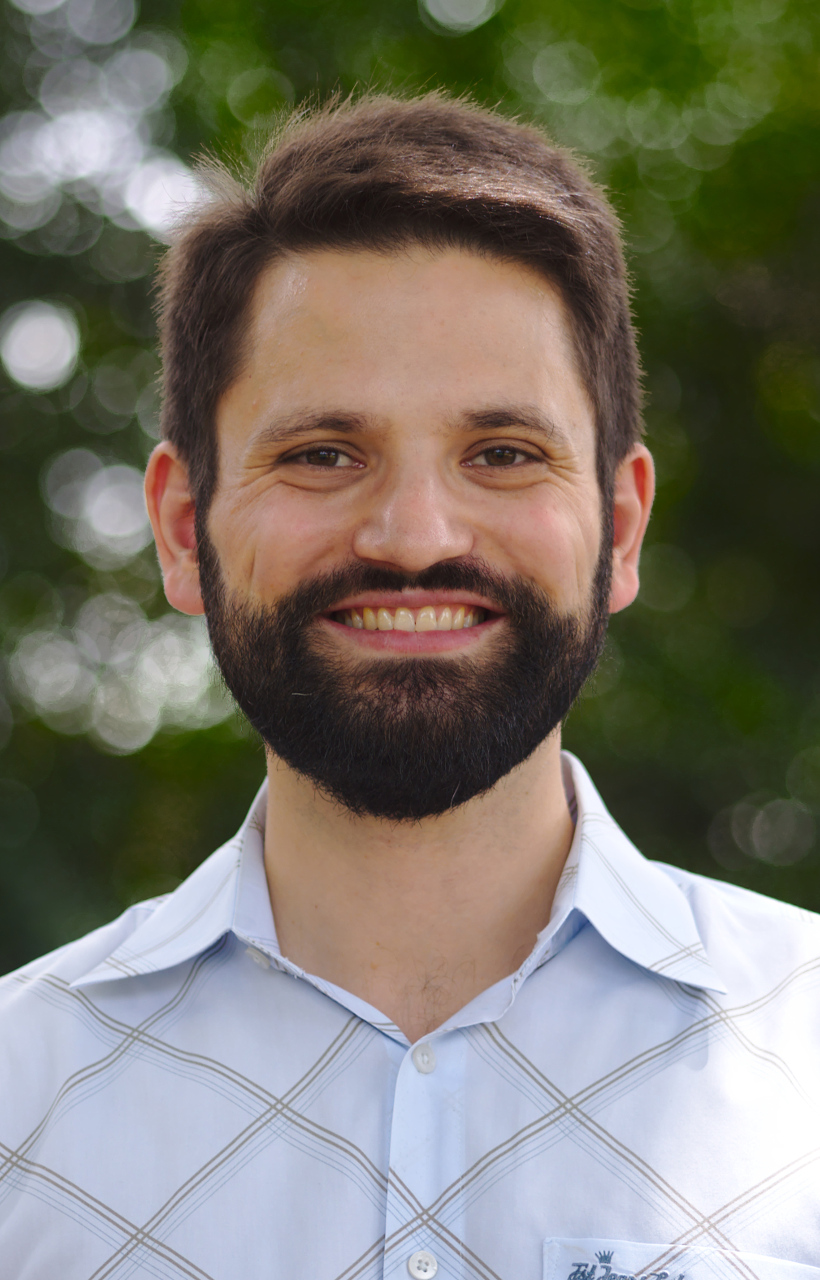
\includegraphics[width=2cm]{joe.jpg}
  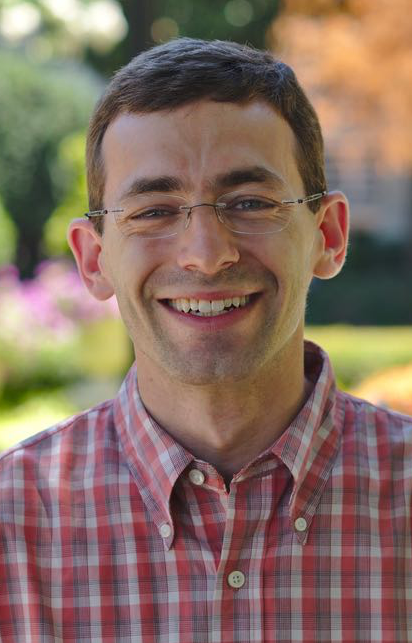
\includegraphics[width=2cm]{dan.png}
};

\vskip5mm
\alert{Math 1553:} Introduction to Linear Algebra
\pause
\begin{itemize}
\item<+-> Largest course in School of Math
\item<+-> Around 2,000 students per year
\item<+-> Majority of all undergrads at Tech
%\item<+-> Almost all engineers
\item<+-> Mostly first-year engineers
\end{itemize}

\pause[6]\vskip1cm
Dan Margalit and I created a textbook that is:
\pause
\begin{itemize}
\item<+-> Specifically targeted to 1553.
%\item<+-> For, by, and about Georgia Tech.
\item<+-> Available online and usable on mobile devices.
\item<+-> Polished, and beautiful to look at.
\item<+-> \alert{Free} 
  \begin{itemize}
  \item<+-> GNU Free Documentation License.
  \item<+-> Source publicly available on \href{https://github.com/QBobWatson/gt-linalg}{\color{green!50!black}GitHub}.
  \end{itemize}
\item<+-> \alert{Interactive}

\end{itemize}

\end{frame}


%%%%%%%%%%%%%%%%%%%%%%%%%%%%%%%%%%%%%%%%%%%%%%%%%%%%%%%%%%%%%%%%%%%

\begin{frame}
\frametitle{Our Motivation}

\vskip-3mm

\hfill\tikz\node[overlay, below left, yshift=1cm, xshift=1cm]{
  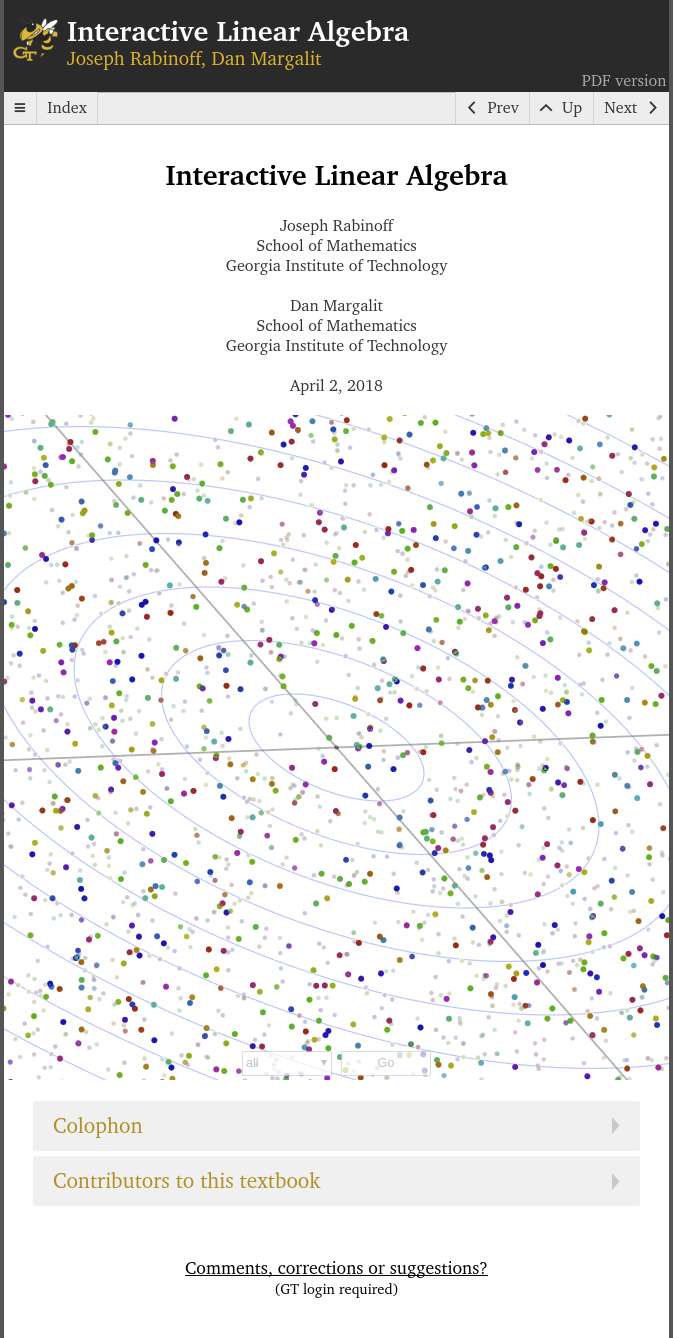
\includegraphics[width=4.5cm]{ila.png}
};

\begin{minipage}{6.5cm}
\alert{Why} write this book?

\pause
\begin{itemize}
\item<+-> Saves students money.
\item<+-> We can do better than the current textbook (Lay).
\item<+-> \alert{Interactive:} First textbook of its kind.
% \item<+-> Georgia Tech paves the way: Creating the Next textbook.
%   \begin{center}
%   
\includegraphics[width=6cm]{cne.jpg}
%   \end{center}
\item<+-> Pedagogical goal: get students to think geometrically.
\item<+-> I want them to \emph{retain} the material by remembering the pictures.

\end{itemize}

\end{minipage}

\end{frame}


%%%%%%%%%%%%%%%%%%%%%%%%%%%%%%%%%%%%%%%%%%%%%%%%%%%%%%%%%%%%%%%%%%%

\begin{frame}
\frametitle{\textit{Interactive} Linear Algebra}

\spalignsysdelims\{.
\alert{Typical Problem:}
\begin{tikzpicture}[anchor=base,baseline]
\node<-4>[draw=white] {\normalsize Describe the solutions};
\node<5->[draw,seq-red] {\normalsize Describe the solutions};
\end{tikzpicture}
of the linear system
\[ \syseq{-2x + 2y - 4z = 6;
            x -  y + 2z = -3}. \]

\pause
Students know the recipe: first make an augmented matrix
\[ 
\amat{-2 2 -4 6; 1 -1 2 -3}
  \quad\longsquiggly[{\demo[interactive]{rrinter.html?mat=-2,2,-4,6:1,-1,2,-3}}]\quad
  \pause
  \amat{1 -1 2 -3; 0 0 0 0}
\]
\note[item]{Want to eliminate some variables.}
\note[item]{Remember how you had to do this on pen and paper\ldots}
\pause
Turn this back into an equation:
\[ x = y - 2z - 3 \]

\note[item]{Students are good at this.}
\note[item]{They think math means recipes that must be mastered.}

\pause\medskip
This slide does \textbf{not} answer the \textcolor{seq-red}{question}.


\end{frame}


%%%%%%%%%%%%%%%%%%%%%%%%%%%%%%%%%%%%%%%%%%%%%%%%%%%%%%%%%%%%%%%%%%%

\begin{frame}
\frametitle{\textit{Interactive} Linear Algebra}

\spalignsysdelims\{.
\alert{Typical Problem:}
\tikz[anchor=base,baseline]\node{\normalsize Describe the solutions};
of the linear system
\[ \syseq{-2x + 2y - 4z = 6;
            x -  y + 2z = -3}. \]

\bigskip
Answer:
\[ 
  x =  y - 2 z - 3
\]

\pause\medskip
I want a \textbf{picture} to immediately pop into the students' heads.

\pause\medskip
Rewrite using matrix notation: $Ax = b$ for
\[ A = \mat{-2 2 -4; 1 -1 2} \qquad b = \vec{6 -3}. \]
\pause
\alert{Question:} What does the set of solutions look like?

\pause\medskip
\alert{Question:} For which $b$ does there exist a solution?

\pause\medskip
\alert{Question:} What happens to the solution set as you vary $b$?

\pause\bigskip
\centering
{\href{http://textbooks.math.gatech.edu/ila/demos/Axequalsb.html?x=-3,0,0&mat=-2,2,-4:1,-1,2&lock=true}{\color{green!50!black}\Large[interactive]}}
\note{Play around with this a bit: unlock solutions, move $x$ and $b$}

\end{frame}


%%%%%%%%%%%%%%%%%%%%%%%%%%%%%%%%%%%%%%%%%%%%%%%%%%%%%%%%%%%%%%%%%%%

\begin{frame}
\frametitle{\textit{Interactive} Linear Algebra}

\alert{Typical Problem:}
Let $A$ be the matrix for reflection over a plane in space.

\pause\medskip
For which points $v$ in space do $Av$ and $v$ lie on the same line through $0$?

\pause\medskip
This is the \textbf{eigenvalue problem}: most important topic.
\note[item]{PageRank from yesterday's lecture.}

\pause\medskip
Students know the recipes for:
\pause
\begin{itemize}
\item<+-> Computing $A$.
\item<+-> Computing the eigenvalues.
\item<+-> Computing eigenvectors for each eigenvalue.
\end{itemize}

\pause[8]\medskip
This is the wrong way to go about answering the question.

\pause\medskip
I want a \textbf{picture} to immediately pop into their heads.
\note[item]{Describe the picture: yellow vector is reflected over green plane.}

\pause\bigskip
\centering
{\href{https://textbooks.math.gatech.edu/ila/demos/eigenspace.html?mat=1/3,-2/3,-2/3:-2/3,1/3,-2/3:-2/3,-2/3,1/3}{\color{green!50!black}\Large[interactive]}}

\end{frame}


%%%%%%%%%%%%%%%%%%%%%%%%%%%%%%%%%%%%%%%%%%%%%%%%%%%%%%%%%%%%%%%%%%%

\begin{frame}
\frametitle{\textit{Interactive} Linear Algebra}

\emph{There are approximately $150$ interactive demonstrations embedded in the text.}

\pause\medskip
Makes abstract linear algebra fundamentally something they can touch and see: first of its kind.

\pause
\begin{itemize}
\item<+-> Highly configurable.
\item<+-> Used exactly like this in lecture too.
\end{itemize}

\pause[5]
\medskip
Made possible by \emph{recent web technologies}: works on any modern browser and on mobile.
\pause
\begin{itemize}
\item<+-> Technology is WebGL.
\item<+-> Framework called Mathbox (Steven Wittens).
\item<+-> About 5,000 lines of Javascript code for demos.
\item<+-> Modified Robert Beezer's Mathbook XML for the text.
\item<+-> Generates online and PDF versions.
\item<+-> I wrote a pdf-to-html converter for the pretty math and the figures.

\end{itemize}

\end{frame}


%%%%%%%%%%%%%%%%%%%%%%%%%%%%%%%%%%%%%%%%%%%%%%%%%%%%%%%%%%%%%%%%%%%

\begin{frame}
\frametitle{Next Steps}

\begin{itemize}
\item<+-> More examples (in progress).
  \begin{center}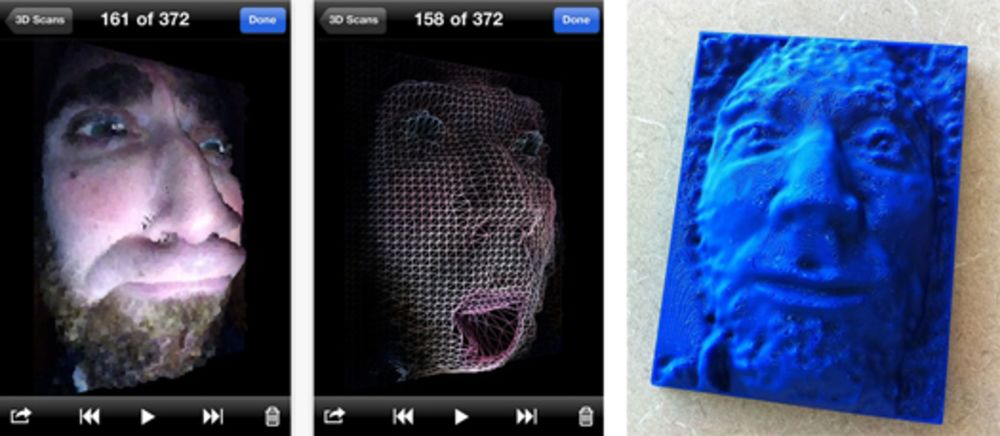
\includegraphics[width=5cm]{trimensional.jpg}\end{center}
  \note{Grant Schindler, CoC, iPhone app using normal vectors.}
\item<+-> More exercises and solutions (in progress).
\item<+-> Expand content to cover similar linear algebra courses (1554).
\item<+-> Other courses can be interactive!  Calculus, DiffEQ, \ldots

\end{itemize}

\end{frame}



%%%%%%%%%%%%%%%%%%%%%%%%%%%%%%%%%%%%%%%%%%%%%%%%%%%%%%%%%%%%%%%%%%%

\begin{frame}
\frametitle{Try It Out}

\centering\huge
\href{https://goo.gl/Tgd73B}{\color{seq-green}\url{https://goo.gl/Tgd73B}}

\bigskip
\huge
\href{https://https://textbooks.math.gatech.edu/ila/}{\color{seq-green}\url{https://textbooks.math.gatech.edu/ila/}}

\end{frame}




\end{document}
